\chapter{PROPOSED SOLUTION}
\label{chap:solution}
\section{Data collecting with crowd-sourcing model}
A traditional method of collecting data is to do it manually : Setting up an array of cameras at desired locations and then obtain their recordings. Those recording would later be labeled by specialists or experts and processed to form a dataset. This way of approach is expensive and requires a lot of human resources.

One other method of data collection is to implement Web crawler to pull data from the internet automatically. This method would be most useful for getting a large amount of data given a keyword. One downside is that data achieved by this method often contain considerable noise because of typos, mislabel or error. In the context of security, those data are not suitable to be used because they are incredibly diverse and do not portray the Vietnamese environment accurately. Moreover, public data used for security matter can be collected by crawler is not considerable or may insufficient.

Crowd-sourcing is also one of the effective methods of data collection which is becoming a trend in the last couple of years. The idea behind crowd-sourcing data is to build datasets with the assistance of the community. An example of this kind of model is Wikipedia\footnotetext{\url:{https://www.wikipedia.org}}
. Wikipedia is an enormous web-based, collaborative encyclopedia which has over 100,000 volunteers contributing new information to the system daily. The success of Wikipedia proves the capability of crowd-sourcing. The solution is applicable to this project due to its advantages of significant cost saving. Furthermore, appropriate datasets can be created by Vietnamese community.

However, how can people be encouraged to provide their knowledge and information? Interaction with others is proven successful in encouraging people to share.Therefore, social media has been a popular trend among Vietnamese in recent years. At the time of November 2018, the amount of people using Facebook has reached about 70 million, that accounts for almost 73\% of the population. (Figure \ref{chap3:social_media_vn}).

\begin{center}
    \begin{figure}[H]
    \centering
    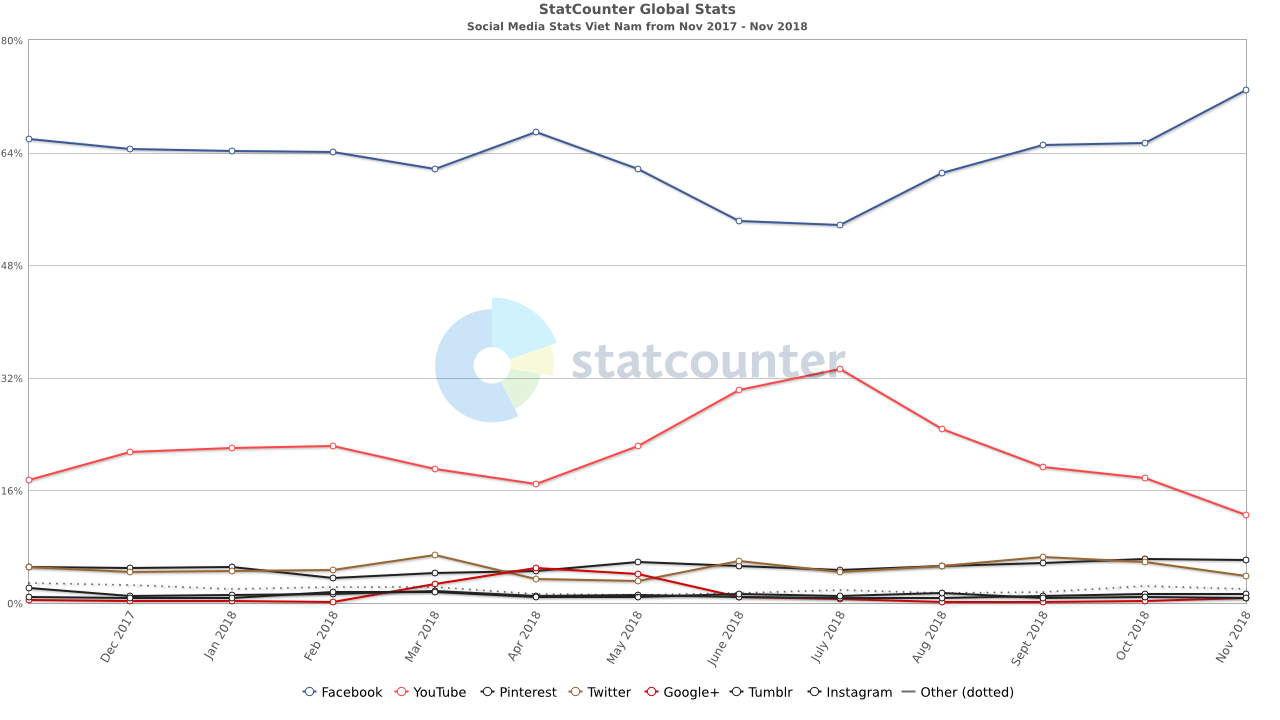
\includegraphics[width=1\columnwidth]{images/chap3/social_media_vn.png}
    \footcaption{Social media usage of Vietnamese is at all time high. Nearly 73\% of the population is using use Facebook}
    \label{chap3:social_media_vn}
    \end{figure}
\end{center}
\vspace{-1cm}
\footnotetext{Source: \url:{http://gs.statcounter.com/social-media-stats/all/viet-nam}}
Because of mentioned factors, this thesis proposes building a \textbf{Social media website for security} where users can interact with each other, as well as provide their data to the system via posting.
\section{Extracting information from images}

For image data, this thesis proposes using a face recognition system to identify faces from photographs. Facial recognition is one of the classical problem in image classification, because of that, there are many companies that offer simple yet effective solutions to this problem through calls to their APIs. There are many ways to recognize faces through APIs such as Kairos, Amazon Recognition, Microsoft Face API, Google Cloud Vision, and IBM Watson Visual Recognition, and these are their features:
\begin{center}
	\begin{figure}[H]
		\centering
		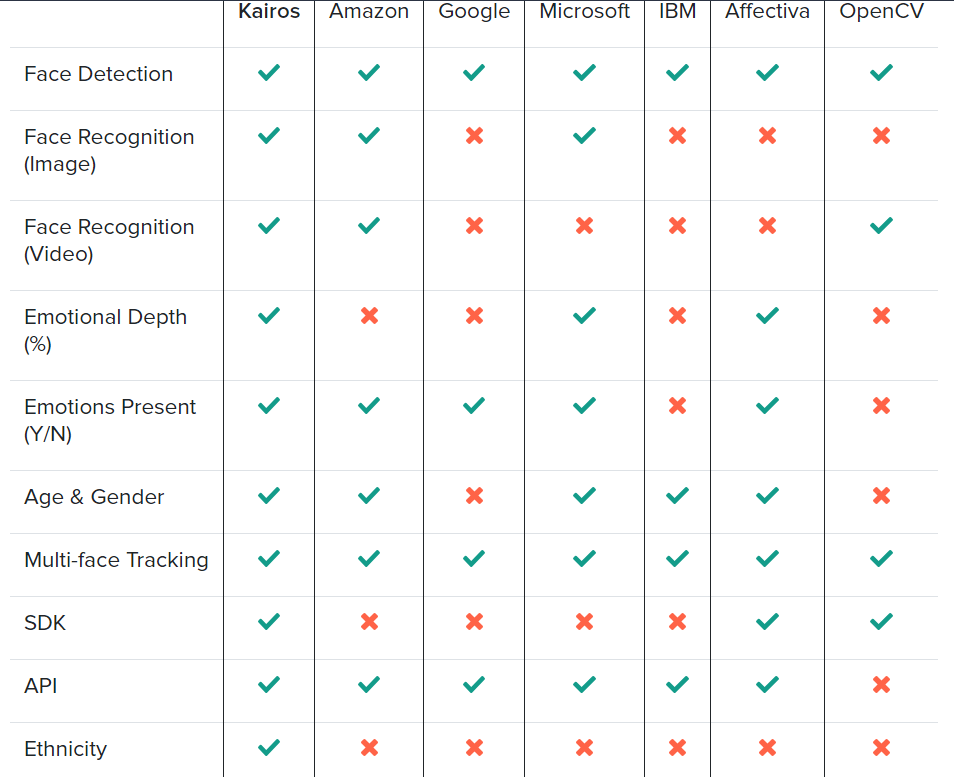
\includegraphics[width=1\columnwidth]{images/chap3/face_api.png}
		\footcaption{Feature of some recent famous facial analyzing services}
		\label{chap3:face_api_now}
	\end{figure}
\end{center}
\footnotetext{Source: \url:{https://www.kairos.com/blog/face-recognition-kairos-vs-microsoft-vs-google-vs-amazon-vs-opencv}}
\begin{itemize}
	\item  Kairos: offers a wide variety of image recognition solutions through their API. Their API endpoints include identifying gender, age, emotional depth, facial recognition in both photo and video, and more.
	\item Amazon Recognition: This facial recognition API is fully integrated into the Amazon Web Service ecosystem. Using this API will make it easy to build applications that make use of other AWS products.
	\item Google Cloud Vision: By being integrated into the Google Cloud Platform, this API will be a breeze to integrate into applications that are already using other Google Cloud Platform products and services.
\end{itemize}

However, with the limitations of the thesis and the applicability to fulfill demands of this research, Microsoft Face API is chosen. There are many advantage of Microsoft Face API such as large amount of user identification, high accuracy and lower cost of usage than the whole API remaining at the time of the investigation


\section{Extracting information from videos}
For the video analyzing problem, this thesis proposes using a two-phased video classification model to find out if there are suspicious behaviors within a video. This model processes videos by passing frames through a Convolutional Neural Network to extract features, then pass the output to a Recurrent Neural Network using LSTM cells, similar to the approach of \cite{DBLP:journals/corr/DonahueHGRVSD14}. This model was trained and test using UCF-101 dataset\footnotetext{Source: url:{http://crcv.ucf.edu/data/UCF101.php}} - A standard dataset commonly used for benchmarking action recognition models - and achieved a moderate result. Figure \ref{chap3:model_architecture} shows the overview of this approach.
\begin{center}
	\begin{figure}[H]
		\centering
		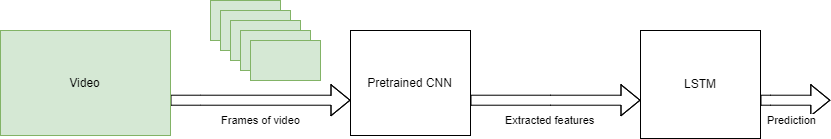
\includegraphics[width=1\columnwidth]{images/chap3/model_architecture.png}
		\caption{Overview of the approach. Videos are separated in to frames and each frame is pass through a pretrained CNN to extract features. Then those features is pass into a LSTM for prediction.}
		\label{chap3:model_architecture}
	\end{figure}
\end{center}
\vspace{-1cm}
\subsection{Proposed Architecture}
\subsubsection{CNN architecture for feature extraction}
In \cite{DBLP:journals/corr/ZhouKLOT14}, the authors suggest that pretrained CNNs are incredibly effective in extracting feature for other classification tasks.
For the CNN layer of the proposal model, VGG16 \cite{DBLP:journals/corr/SimonyanZ14a} architecture and Resnet50 architecture pretrained on ImageNet \footnotetext{Source: \url:{http://www.image-net.org/challenges/LSVRC/}} is chosen to extract features from video frames. Figure \ref{chap3:vgg16_architecture} shows the architecture of VGG16 model. Input of VGG16 is an 224x224x3 RGB image. The image is then pass through a stack of convolutional layers. All of hidden layers are equipped with a ReLU.\\
Each video will be split into frames, these frames will go through VGG16 for the purpose of extracting features. After passing the network, extracted features are tensors with the shape (7x7x512).
\begin{center}
    \begin{figure}[H]
    \centering
    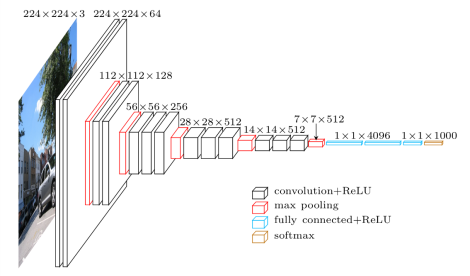
\includegraphics[width=1\columnwidth]{images/chap3/vgg16_architecture.png}
    \footcaption{Architecture of the VGG16 CNN}
    \label{chap3:vgg16_architecture}
    \end{figure}
\end{center}
\footnotetext{Source: \url:{https://blog.heuritech.com/2016/02/29/a-brief-report-of-the-heuritech-deep-learning-meetup-5/}}
\vspace{-1cm}
\subsubsection{LSTM for sequence learning}
Output of VGG16 is passed through LSTM cells for prediction.
LSTM in Keras takes input with shape (\textit{number-of-sample, number-timesteps, number-features}).
\begin{itemize}
	\item Number of sample could be any positive number.
	\item Number timesteps is the number of sequential data (frame) as a single sample.
	\item Number features is a shape of features extract from VGG16. In this case, it's equal to 25088 = 7x7x512.
\end{itemize}

\begin{center}
	\begin{figure}[H]
		\centering
		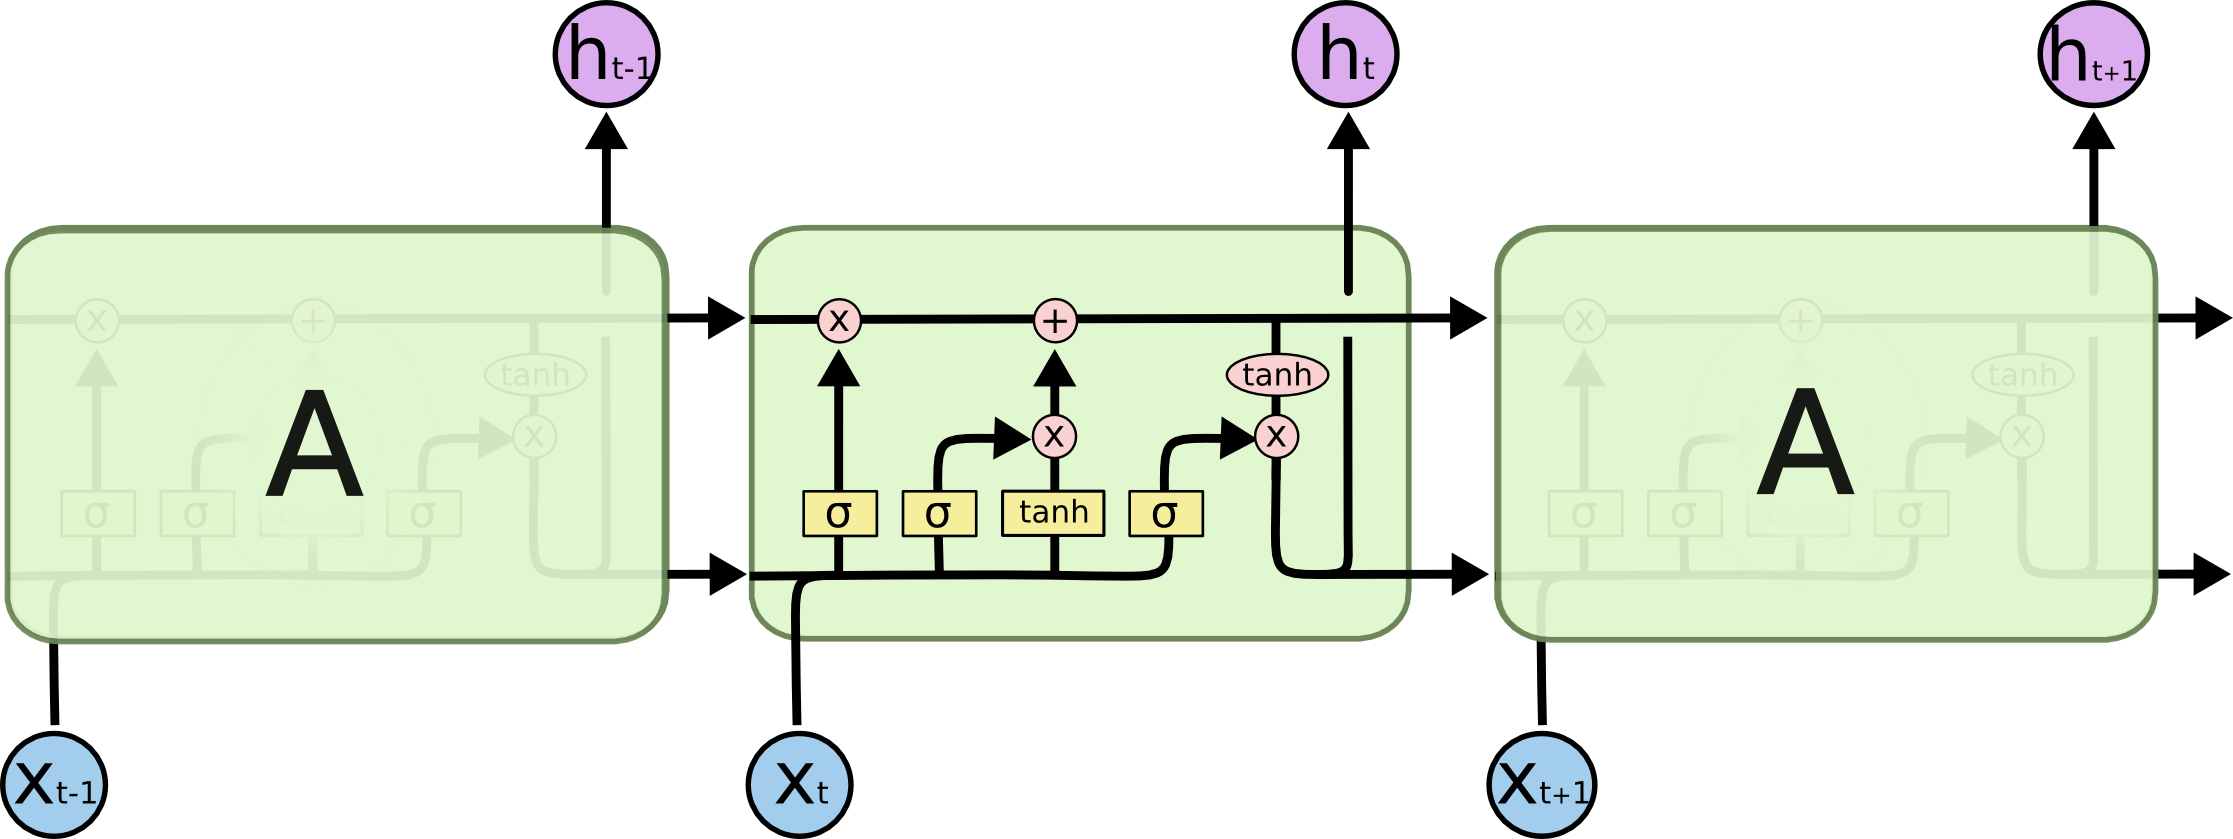
\includegraphics[width=1\columnwidth]{images/chap3/lstm-chain.png}
		\caption{Long short-term memory in Keras}
		\label{chap3:lstm-chain}
	\end{figure}
\end{center}

\subsection{Dataset}
\textbf{UCF101} \footnotetext{Source: \url{http://crcv.ucf.edu/data/UCF101.php}} was used to evaluate this model. It is a standard dataset used for testing action recognition models. This dataset comprise of 13320 videos divided into 101 action categories collected from the Youtube website.
There are some summary about UCF-101 Dataset:
\begin{center}
	\begin{figure}[H]
		\centering
		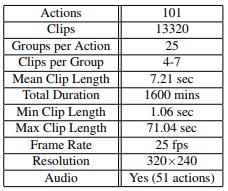
\includegraphics[width=0.4\columnwidth]{images/chap3/ucf-sum.png}
		\footcaption{Summary of characteristics of UCF-101 Dataset}
		\label{chap3:ucf-sum}
	\end{figure}
\end{center}
\begin{center}
	\begin{figure}[H]
		\centering
		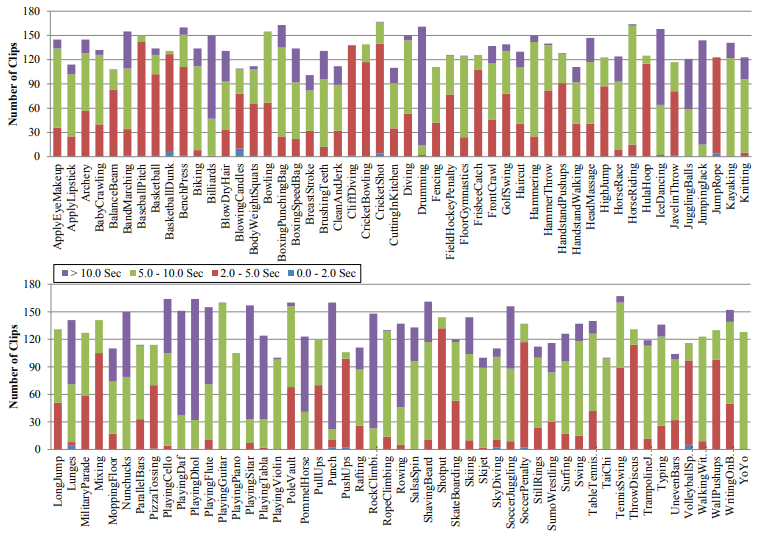
\includegraphics[width=1\columnwidth]{images/chap3/ucf-sum-chart-2.png}
		\caption{Number of clips per action class. The distribution of clip durations is illustrated by the colors}
		\label{chap3:ucf-sum-chart-2}
	\end{figure}
\end{center}
% \subsection{Evaluating}

\subsection{Preprocessing}
As mentioned before, videos would mostly come from smartphones. A video came from a smartphone could come in many orientations. Because of that, it would have \textbf{metadata} containing orientation data, making it rotate. Despite that, traditional computer vision libraries like OpenCV cannot read metadata from videos, making those videos inaccurate for training. Because of that, \textbf{FFprobe}\footnotetext{Source: \url{https://www.ffmpeg.org/ffprobe.html}} is used to extract metadata from videos.\\
For every video, a subprocess with the following command below would launch to extract the rotational info :\\
\begin{center}
\textit{ffprobe -loglevel error -select\_streams v:0 -show\_entries stream\_tags=rotate -of  default=nw=1:nk=1 video\_file\_name}
\end{center}
After that, depending on the orientation of the video is 0, 90, 180 or 270, each frame would be rotated by the corresponding angle before inputting into the CNN for extracting feature. 
\subsection{Hyperparameter}
The table below shows hyperparameters used in the model.
\begin{table}[H]
	\begin{tabular}{|P{5cm}|L{5cm}|}
		\hline
		\textbf{Name}				&  \textbf{Value}
		\\ \hline
		Hidden units in LSTM		&   1024
		\\ \hline
		Dropout	in LSTM				&  	0.6      
		\\ \hline
		Dropout after Dense layer	&	0.5
		\\ \hline
		Number of frames			&   14
		\\ \hline
		Batch size					&   256
		\\ \hline
		Epochs						&   20
		\\ \hline
		Learning rate				&   0.001
		\\ \hline
	\end{tabular}
\caption{Hyperparameters used}
Accuracy of the model achieved an acceptable result after 20 epochs.
\end{table}
\subsection{Training method}
For training this model,\textbf{RMSprop} optimizer is used with Learning Rate is 0.001. On the other hand, a Dropout layer is used with 0.5 proportion for avoiding an overfitting problem. The dataset is divided into 2 part: 80\% for training and validation, 20\% for testing. For training and validation, an 8 to 2 porpotion is also applied. The model is trained for 20 epochs and apply early stopping. The chosen model is model which has the highest accuracy in the validation set.The figure below shows the training process of the chosen model. For the optimization of a model which is not overfit or underfit, both Train Accuracy and Validation Accuracy have the tendency of increasing, while Train Loss and Validation Loss have tendency of decreasing.
 
\begin{center}
	\begin{figure}[H]
		\centering
		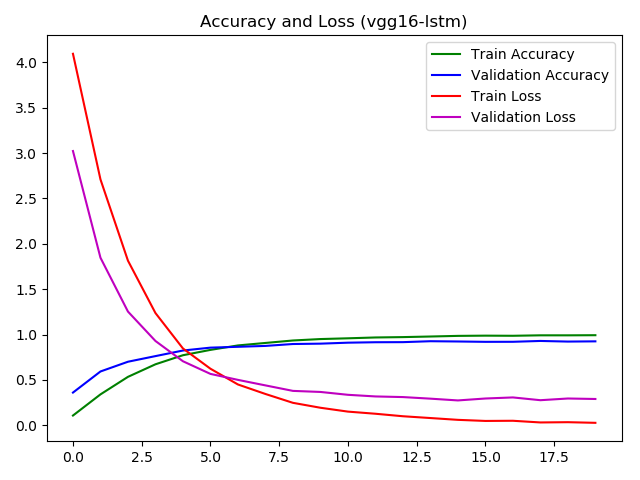
\includegraphics[width=0.8\columnwidth]{images/chap3/acc-and-loss.png}
		\footcaption{Training process of VGG16 + LSTM model}
		\label{chap3:acc-and-loss}
	\end{figure}
\end{center}
\subsection{Result}
There are many methods to evaluate classification models depending on the problem. Commonly used methods are: accuracy score, confusion matrix, Curve Under Area, Precision and Recall, F1 score. For multi-class classification problems, if the data is relatively uniformly distributed, the two well-known methods commonly used are \textbf{Confusion matrix} and \textbf{Accuracy}.\\ 
\textbf{Accuracy} is the amount of correct predictions over the total number of prediction.\\
In a Confusion matrix, each \textbf{row} is the value of the \textbf{correct label} and each \textbf{column} is the label \textbf{predicted} by the model. Each number at the intersection between each row and column is the proportion that the video has the label as the value at the row predicted to be the label at the column.\\
\begin{center}
	\begin{figure}[H]
		\centering
		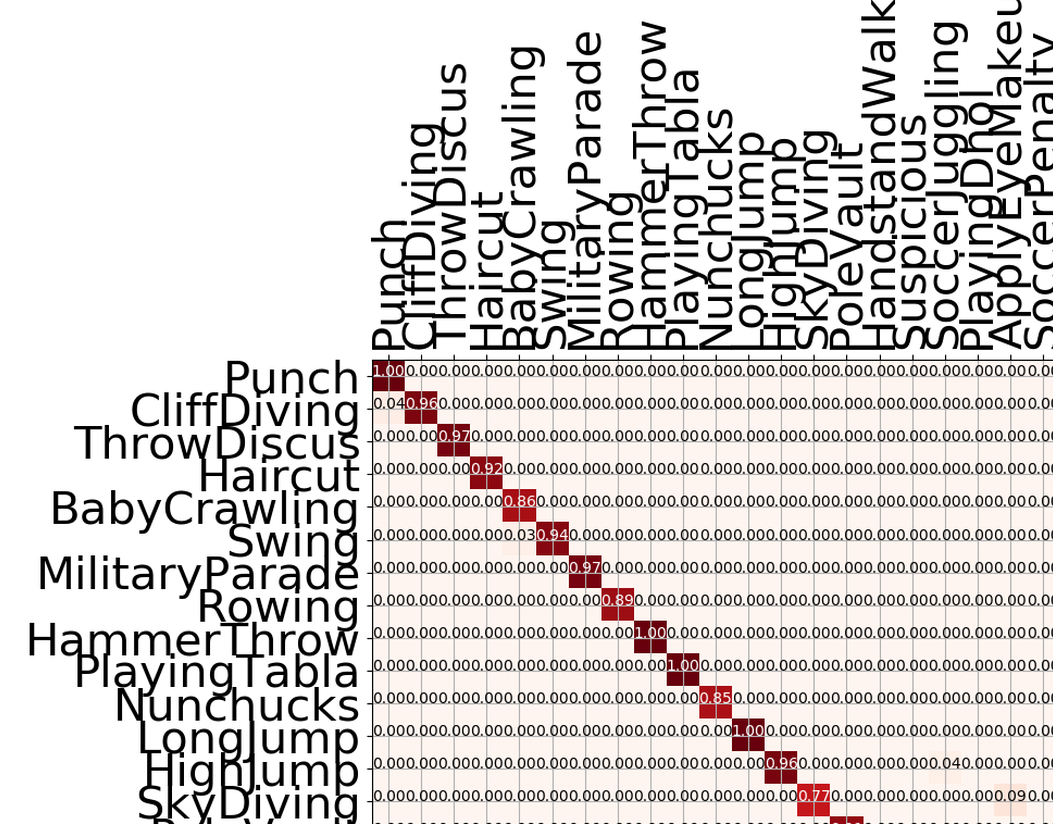
\includegraphics[width=1\columnwidth]{images/chap3/CFM-zoom.png}
		\caption{Detail in Confusion Matrix of VGG16 + LSTM model}
		\label{chap3:cfm-zoom}
	\end{figure}
\end{center}
\vspace{-1cm}
For example, there are 82\% IceDancing videos is predicted as IceDancing, 9\% of IceDancing videos is predicted as Haircut.\\
Furthermore, the intersection cells are also indicated in red color, with the value increasing gradually from 0 to 1, the density of the color will change accordingly, from light red to dark red.\\
A good model that will give a confusion matrix has elements on the main diagonal line that have a large value, the remaining elements have small values. In other words, when representing Confusion Matrix in color, a good model will have a main diagonal that will be darker than other areas.
\begin{center}
	\begin{figure}[H]
		\centering
		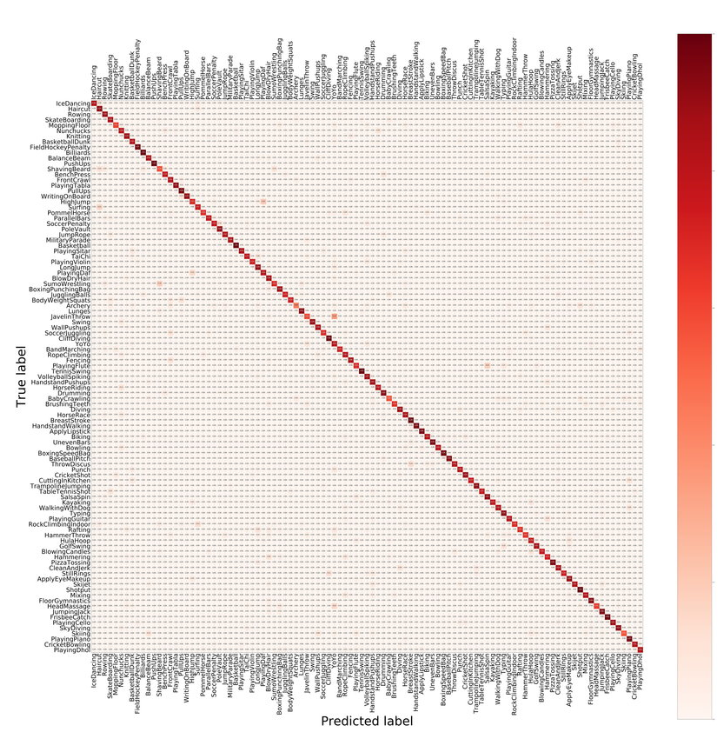
\includegraphics[width=1\columnwidth]{images/chap3/cfm-2.jpg}
		\caption{Confusion Matrix of VGG16 + LSTM model}
		\label{chap3:cfm-zoom}
	\end{figure}
\end{center}
\vspace{-1cm}
The table below show accuracy of tested models.
\begin{table}[H]
	\begin{tabular}{|P{5cm}|L{5cm}|}
		\hline
		\textbf{Model name}			&  \textbf{Accuracy}(After 20 epochs)
		\\ \hline
		VGG16+LSTM	 	&   ~91.8\%  
		\\ \hline
		Resnet+LSTM 	&  	90.2\%       
		\\ \hline
	\end{tabular}
\caption{Accuracy of the tested models}
\end{table}



